\documentclass[conference]{IEEEtran}
\IEEEoverridecommandlockouts
\usepackage{cite}
\usepackage{amsmath,amssymb,amsfonts}
\usepackage{algorithmic}
\usepackage{graphicx}
\graphicspath{{./}{../docs/}{docs/}}
\usepackage{textcomp}
\usepackage{xcolor}
\usepackage{booktabs}
\usepackage{bm}
\usepackage{url}

\def\BibTeX{{\rm B\kern-.05em{\sc i\kern-.025em b}\kern-.08em
    T\kern-.1667em\lower.7ex\hbox{E}\kern-.125emX}}

\begin{document}

\title{Route Diversity and Exploitability in Competitive Multi-Agent Reinforcement Learning}

\author{
\IEEEauthorblockN{Navadeep Nindra}
\IEEEauthorblockA{\textit{Department of Mathematics} \\
\textit{SVNIT Surat}, India \\
u24mc006@amhd.svnit.ac.in}
\and
\IEEEauthorblockN{Brij Radadiya}
\IEEEauthorblockA{\textit{Department of Mathematics} \\
\textit{SVNIT Surat}, India \\
u24mc005@amhd.svnit.ac.in}
\and
\IEEEauthorblockN{Shrey Marakana}
\IEEEauthorblockA{\textit{Department of Mathematics} \\
\textit{SVNIT Surat}, India \\
u24mc009@amhd.svnit.ac.in}
\and
\IEEEauthorblockN{Shree Pastagia}
\IEEEauthorblockA{\textit{Department of Mathematics} \\
\textit{SVNIT Surat}, India \\
u24mc012@amhd.svnit.ac.in}
}

\maketitle

\begin{abstract}
In multi-agent reinforcement learning (MARL), agents learn while affecting one another. In self-play, each agent faces an opponent that is also changing, so a route that worked before may stop working. This paper studies that problem in the Three Bridges Arena, a grid game where an Attacker crosses one of three bridges to reach a target while a Defender tries to catch it. We compare direct self-play with Dual-Archive Co-Evolution, which also trains agents against saved versions of earlier opponents. The agents use symmetric potential-based reward shaping with a discount factor of 0.99; this keeps the shaping rewards for the two players equal and opposite. In 150 paired evaluations, direct self-play used the North bridge in 46.0 percent of crossings and the South bridge in 16.1 percent, and 17.3 percent of episodes timed out. The archive-trained policy had route entropy of 1.567 bits, or 98.9 percent of the maximum for three routes, and no timeouts in this evaluation. Its measured exploitability was 0.140, compared with 0.160 for direct self-play. The worst-case security score changed from -0.207 to -0.187. The pooled win-rate difference was -0.6 percent and was not statistically significant. These results suggest that route use and exploitability can help compare strategies. They do not directly test whether an agent has forgotten a previously learned route.
\end{abstract}

\begin{IEEEkeywords}
Multi-Agent Reinforcement Learning, Self-Play, Route Diversity, Exploitability, Potential-Based Reward Shaping, Zero-Sum Games.
\end{IEEEkeywords}

\section{Introduction}
In multi-agent reinforcement learning (MARL), several decision-making agents act in the same environment. In self-play, agents learn by playing against one another. Each agent changes its behavior as it learns, so the opponent is also changing during training. Self-play has produced strong results in games such as Go, StarCraft, and Dota 2 \cite{silver2016mastering, vinyals2019alphastar, berner2019dota}.

When both agents learn at the same time, each agent faces a changing opponent. Researchers call this a non-stationary learning problem. In some games, strategies can cycle: one behavior is answered by another, which is later answered in turn. This pattern is sometimes compared with the Red Queen effect \cite{balduzzi2019open, cliff1995tracking}. The comparison is an analogy; this grid game is not a biological model.

A related concern is catastrophic forgetting: a neural network may lose an earlier skill while learning a new one \cite{mccloskey1989catastrophic}. In this project, we use bridge choices as an indirect measure of route diversity. A change in route frequency alone does not prove that an agent has forgotten how to use a route.

We study these questions in the \textit{Three Bridges Arena}, a two-player grid game. The Attacker tries to cross a river and reach a target. The Defender tries to catch the Attacker before it arrives. Four blocked cells leave three possible crossings: North, Center, and South. Since one Defender cannot stand at all three crossings at once, the Attacker has more than one possible route.

This paper describes the arena, compares self-play with archive training, and reports the following measurements:
\begin{enumerate}
    \item \textbf{Game and reward design:} We describe the grid game and use symmetric reward shaping. The two shaping rewards are equal in size and opposite in sign, so their sum is zero. Earlier work gives conditions under which potential-based shaping preserves policies or equilibria (Ng et al. \cite{ng1999policy}; Devlin and Kudenko \cite{devlin2011theoretical}).
    \item \textbf{Dual-Archive Co-Evolutionary Framework:} We implement a symmetric multi-agent architecture maintaining persistent historical snapshot reservoirs for both Attacker and Defender. Policies train on a tripartite mixture of active self-play (60\%), active Attacker vs. archived Defender (20\%), and archived Attacker vs. active Defender (20\%).
    \item \textbf{Route diversity measurement:} We use Shannon entropy to summarize how evenly successful crossings are spread across the three bridges. This describes route use; it is not a direct test of forgetting.
    \item \textbf{Empirical Game-Theoretic Analysis (EGTA):} We construct a spatial meta-game payoff matrix against an archetypal adversary suite, computing empirical minimax game values, security levels ($v_{\text{sec}}$), and exploitability distances ($\delta$).
    \item \textbf{Evaluation:} In 150 paired evaluations, the archive-trained policy used the three routes more evenly and had fewer timeouts than the direct self-play policy. Its measured exploitability was 0.140 versus 0.160, and its worst-case security score was -0.187 versus -0.207. These results are limited to the policies and opponents tested here.
\end{enumerate}

\section{Related Work}

\subsection{Self-Play and Policy Cycling in MARL}
Self-play training traces back to TD-Gammon \cite{tesauro1995temporal} and has been central to modern multi-agent milestones \cite{silver2016mastering, vinyals2019alphastar, berner2019dota}. However, theoretical analysis shows that independent gradient ascent in multi-agent systems often diverges or enters limit cycles in games with intransitive dynamics \cite{balduzzi2019open}. Cliff and Miller \cite{cliff1995tracking} characterized this phenomenon in co-evolutionary algorithms as the Red Queen dynamic. Without memory or population diversity, agents continuously chase moving targets without making genuine global progress.

\subsection{Memory Reservoirs, Double Oracle, and PSRO}
Game theory addresses policy cycling through Fictitious Play \cite{brown1951iterative}, in which players best-respond to the empirical average strategy of their opponent's historical actions. In high-dimensional policy spaces, the Double Oracle algorithm \cite{mcmahan2003planning} iteratively computes minimax equilibria over restricted strategy sets. Lanctot et al. \cite{lanctot2017unified} generalized this concept to deep reinforcement learning via Policy-Space Response Oracles (PSRO), where reinforcement learning oracles generate best responses against mixed meta-strategies. Neural Fictitious Self-Play (NFSP) \cite{heinrich2016deep} similarly utilizes transition replay buffers to approximate fictitious play in extensive-form games. 

While landmark architectures such as AlphaStar \cite{vinyals2019alphastar} deploy vast, asymmetrical league-training frameworks involving main agents and specialized exploiter agents, such setups require prohibitive compute infrastructure. Our Dual-Archive framework introduces a symmetrical, lightweight snapshot reservoir specifically tailored for two-player zero-sum spatial interactions.

\subsection{Potential-Based Reward Shaping in Zero-Sum Games}
Reward sparsity is an acute challenge in multi-agent navigation. Potential-Based Reward Shaping (PBRS), introduced by Ng et al. \cite{ng1999policy}, guarantees that adding a difference of potentials $F(s, s') = \gamma \Phi(s') - \Phi(s)$ preserves the set of optimal policies in single-agent Markov Decision Processes. Devlin and Kudenko \cite{devlin2011theoretical} extended PBRS to multi-agent stochastic games, showing that if shaping is applied symmetrically such that $\sum_{i} F_i(s, s') = 0$, the zero-sum structural invariant is preserved and the underlying Nash equilibria remain intact.

\section{Game Formulation and Theoretical Framework}

\subsection{Two-Player Zero-Sum Markov Game Formalism}
We formulate the competitive spatial interaction as a discrete-time, two-player zero-sum Markov game defined by the tuple:
\begin{equation}
\mathcal{M} = \langle \mathcal{S}, \mathcal{A}_1, \mathcal{A}_2, \mathcal{P}, \mathcal{R}_1, \mathcal{R}_2, \gamma \rangle
\end{equation}
where:
\begin{itemize}
    \item $\mathcal{S} \subset [0, 1]^6$ is the continuous normalized observation space representing the spatial coordinates of both agents and the objective target.
    \item $\mathcal{A}_1, \mathcal{A}_2$ are discrete action spaces for Player 1 (Attacker) and Player 2 (Defender), each of cardinality $|\mathcal{A}_i| = 5$.
    \item $\mathcal{P}: \mathcal{S} \times \mathcal{A}_1 \times \mathcal{A}_2 \to \Delta(\mathcal{S})$ denotes the deterministic state transition probability distribution governed by the grid dynamics.
    \item $\mathcal{R}_1, \mathcal{R}_2: \mathcal{S} \times \mathcal{A}_1 \times \mathcal{A}_2 \to \mathbb{R}$ are the scalar reward functions satisfying the strict zero-sum condition $\mathcal{R}_1(s, a_1, a_2) + \mathcal{R}_2(s, a_1, a_2) = 0, \forall s, a_1, a_2$.
    \item $\gamma \in [0, 1)$ is the temporal discount factor, set to $\gamma = 0.99$.
\end{itemize}

\subsection{Spatial Topology: The Three Bridges Arena}
The game is instantiated on a 2D discrete coordinate lattice of dimensions $W = 11$ ($X \in \{0, \dots, 10\}$) and $H = 7$ ($Y \in \{0, \dots, 6\}$). The arena is partitioned longitudinally by a river barrier located at column $X = 5$:
\begin{itemize}
    \item \textbf{Infiltration Basin ($X \in [0, 4]$):} The Attacker spawns uniformly across coordinates $X_A \in [0, 3], Y_A \in [0, 6]$.
    \item \textbf{River Barrier ($X = 5$):} The column contains four impassable terrain pillars at $(5, 0), (5, 2), (5, 4), (5, 6)$ and three passable bridge apertures:
    \begin{align}
    \text{North Bridge:} \quad & b_N = (5, 1) \\
    \text{Center Bridge:} \quad & b_C = (5, 3) \\
    \text{South Bridge:} \quad & b_S = (5, 5)
    \end{align}
    \item \textbf{Defensive Basin ($X \in [6, 10]$):} The Defender spawns uniformly across coordinates $X_D \in [6, 9], Y_D \in [0, 6]$ (excluding the Citadel cell).
    \item \textbf{Citadel Target:} A static terminal capture objective located at $(X_T, Y_T) = (10, 3)$.
\end{itemize}

\subsection{State Representation and Action Dynamics}
The global state observation $s_t \in \mathcal{S}$ is normalized over coordinate dimensions $(W-1)$ and $(H-1)$:
\begin{equation}
s_t = \left[ \frac{x_A}{10}, \frac{y_A}{6}, \frac{x_D}{10}, \frac{y_D}{6}, \frac{x_T}{10}, \frac{y_T}{6} \right]^T
\end{equation}
Normalizing by maximal indices guarantees $s_t \in [0, 1]^6$, stabilizing neural value baseline updates.

At each discrete time step $t$, agents execute actions simultaneously from the discrete set $\mathcal{A} = \{\text{UP}, \text{DOWN}, \text{LEFT}, \text{RIGHT}, \text{STAY}\}$. Transitions obey:
\begin{equation}
\bm{p}_{i, t+1} = \bm{p}_{i, t} + \bm{v}(a_{i, t})
\end{equation}
subject to boundary constraints $0 \le x < 11$, $0 \le y < 7$, and obstacle exclusion $(x, y) \notin \{(5, 0), (5, 2), (5, 4), (5, 6)\}$. Attempts to breach boundary walls or impassable pillars result in zero displacement ($\bm{p}_{i, t+1} = \bm{p}_{i, t}$).

\subsection{Terminal Conditions and Mutual Priority}
An episode terminates immediately upon the occurrence of any of the following mutually exclusive conditions:
\begin{enumerate}
    \item \textbf{Citadel Infiltration:} The Attacker occupies the Citadel cell ($\bm{p}_A = (10, 3)$). The terminal payoffs are $R_A = +10, R_D = -10$.
    \item \textbf{Interception / Capture:} The Defender intercepts the Attacker prior to Citadel entry. Interception occurs if $\bm{p}_{A, t+1} = \bm{p}_{D, t+1}$ (co-location) or $\bm{p}_{A, t+1} = \bm{p}_{D, t} \land \bm{p}_{D, t+1} = \bm{p}_{A, t}$ (crossing-swap capture). The terminal payoffs are $R_A = -10, R_D = +10$.
    \item \textbf{Horizon Truncation:} Elapsed time steps reach $T_{\max} = 75$ without Citadel reach or interception. The terminal payoffs are $R_A = 0, R_D = 0$.
\end{enumerate}
Terminal priority is strictly enforced: if the Attacker reaches $(10, 3)$ simultaneously with Defender interception, Citadel capture takes absolute priority ($\text{caught} = \text{raw\_caught} \land \neg \text{reached\_target}$), eliminating ambiguous dual-win credit assignment.

\subsection{A Simplified Three-Route Matching Model}
To illustrate why mixing routes can matter, we analyze a simplified matching model. It treats the three routes as the only choices and assigns a fixed payoff for matching or missing the defended route. The result below applies to that model, not automatically to every state and movement in the full grid game. Let $S_A = \{b_N, b_C, b_S\}$ and $S_D = \{g_N, g_C, g_S\}$ denote the abstract pure route choices for Attacker traversal and Defender bottleneck guarding. The Defender has speed parity with the Attacker ($1 \text{ cell/step}$) and occupies exactly one coordinate. The Manhattan transit distance between outer bridges $b_N$ and $b_S$ is 4 steps, whereas an Attacker at the river barrier can transit across the river in a single forward step. Consequently:
\begin{equation}
\forall s_D \in S_D, \quad \exists s_A \in S_A \quad \text{s.t.} \quad \mathcal{P}(\text{breach} \mid s_A, s_D) = 1.0
\end{equation}
If the Defender commits to guarding $b_N$, the Attacker exploits $b_S$. If the Defender moves to $b_S$, the Attacker shifts to $b_C$ or $b_N$.

\textbf{Result for the simplified model:} \textit{The three-route matching payoff matrix below has no pure-strategy equilibrium. Its minimax strategy chooses each route with probability $\frac{1}{3}$. This result is about the simplified matrix model only.}

\textit{Proof Sketch:} Consider the $3 \times 3$ zero-sum matching game where the Defender successfully intercepts if choosing the identical bridge, earning payoff $+1$, while the Attacker breaches if choosing an unguarded bridge, earning payoff $-1$ for the Defender. The payoff matrix $M_D$ for the Defender is:
\begin{equation}
M_D = \begin{bmatrix} +1 & -1 & -1 \\ -1 & +1 & -1 \\ -1 & -1 & +1 \end{bmatrix}
\end{equation}
For any pure strategy $e_i$, $\min_j (e_i^T M_D)_j = -1$. For the uniform mixed strategy $\bm{q}^* = [\frac{1}{3}, \frac{1}{3}, \frac{1}{3}]^T$, the expected payoff against any pure Attacker action $j$ is $\bm{q}^{*T} M_D e_j = \frac{1}{3}(+1) + \frac{2}{3}(-1) = -\frac{1}{3}$. By the Minimax Theorem \cite{von1944theory}, the value of the game is $v^* = -\frac{1}{3}$, uniquely satisfied by $\bm{p}^* = \bm{q}^* = [\frac{1}{3}, \frac{1}{3}, \frac{1}{3}]^T$. \hfill $\blacksquare$

\subsection{Zero-Sum Discounted Potential-Based Reward Shaping}
Because sparse terminal rewards ($\pm 10$ at $t \le 75$) induce high policy variance and sluggish early exploration, we integrate continuous potential-based reward shaping.

The target distance potential $D_A(x, y)$ is defined piecewise across the river:
\begin{equation}
D_A(x, y) = \begin{cases} 
\min_{b_y \in \{1, 3, 5\}} \left( |x - 4| + |y - b_y| + 6 + |b_y - 3| \right), & x \le 4 \\
|x - 10| + |y - 3|, & x > 4
\end{cases}
\end{equation}
The additional term $|b_y - 3|$ accounts for the vertical distance from each bridge exit to the Citadel centerline ($y=3$), ensuring exact step-wise distance monotonicity across all three bridge corridors. Under discount factor $\gamma = 0.99$, the target-advance shaping component is:
\begin{equation}
F_{\text{tgt}}(s, s') = \alpha_{\text{tgt}} \left[ D_A(s) - \gamma D_A(s') \right]
\label{eq:shaping_tgt}
\end{equation}
where $\alpha_{\text{tgt}} = 0.3$.

To balance offensive progression with tactical interception, we include a relative pursuit-evasion shaping potential $D_{\text{rel}}(s) = |x_A - x_D| + |y_A - y_D|$ with scaling factor $\alpha_{\text{rel}} = 0.2$:
\begin{equation}
F_{\text{rel}}(s, s') = \alpha_{\text{rel}} \left[ D_{\text{rel}}(s) - \gamma D_{\text{rel}}(s') \right]
\label{eq:shaping_rel}
\end{equation}
The joint shaping rewards for Attacker and Defender are formulated symmetrically:
\begin{align}
F_A(s, s') &= +F_{\text{tgt}}(s, s') - F_{\text{rel}}(s, s') \\
F_D(s, s') &= -F_{\text{tgt}}(s, s') + F_{\text{rel}}(s, s')
\end{align}
Because $F_A(s, s') + F_D(s, s') \equiv 0.000000$ identically at every transition, total reward satisfies:
\begin{equation}
R_A(s, a_1, a_2) + R_D(s, a_1, a_2) \equiv 0.000000, \quad \forall s, s' \in \mathcal{S}
\end{equation}
By Devlin and Kudenko \cite{devlin2011theoretical}, symmetric potential shaping does not alter the Nash equilibrium strategy set of the underlying stochastic game.

% The detailed multi-target extension appears in Section VII.

\begin{figure}[t]
\centering
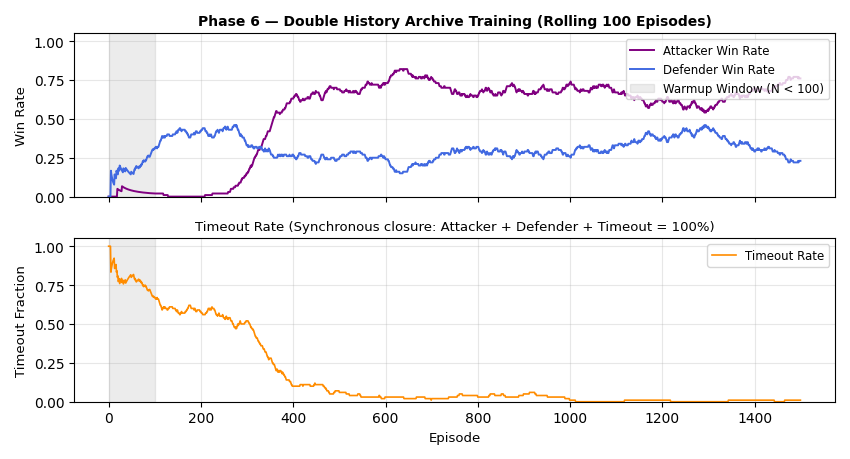
\includegraphics[width=0.92\columnwidth]{phase6_archive_curve.png}
\caption{Dual-Archive training dynamics across 1,500 episodes. Top: Rolling win rates for Attacker (purple, stabilizing near $\approx 65\%$) and Defender (blue, stabilizing near $\approx 33\%$), reflecting the inherent structural advantage of 3 bridges against 1 defender. Bottom: Decline in episode timeout rate from $\approx 80\%$ during initial exploration to below 2\% at convergence.}
\label{fig:training_curve}
\end{figure}

\section{Dual-Archive Co-Evolutionary Framework}

\subsection{The Vulnerability of Unanchored Self-Play}
In standard self-play (Phase 4), parameter vectors $\theta_A$ and $\theta_D$ are optimized directly against each other:
\begin{align}
\theta_{A, k+1} &\leftarrow \theta_{A, k} + \eta_A \nabla_{\theta_A} \mathcal{J}_A(\theta_{A, k}, \theta_{D, k}) \\
\theta_{D, k+1} &\leftarrow \theta_{D, k} + \eta_D \nabla_{\theta_D} \mathcal{J}_D(\theta_{A, k}, \theta_{D, k})
\end{align}
Because gradient updates occur concurrently, neither policy provides a stationary distribution. When $\theta_{A}$ learns to breach the North bridge, $\theta_D$ adapts exclusively to defend the North choke point. In response, $\theta_A$ pivots to the South bridge, discarding its ability to navigate North or Center. This non-stationarity leads to cyclical trajectory collapse.

\subsection{Dual-Archive Architecture}
To anchor learning without requiring vast league-training infrastructure, we implement a symmetric Dual-Archive framework (Phase 6). We maintain two historical model reservoirs:
\begin{equation}
\mathcal{H}_A = \{\pi_A^{(1)}, \pi_A^{(2)}, \dots, \pi_A^{(K)}\}, \quad \mathcal{H}_D = \{\pi_D^{(1)}, \pi_D^{(2)}, \dots, \pi_D^{(K)}\}
\end{equation}
where snapshots of the active policy networks are frozen and appended to the respective archive every $E_{\text{snap}} = 100$ episodes following a warm-up period of $E_{\text{warm}} = 300$ episodes.

During episode rollout, opponents are sampled according to a symmetric tripartite scheme:
\begin{itemize}
    \item \textbf{Active Co-Evolution (60\%):} The active Attacker plays against the active Defender. Both policies gather rollout buffers and update their neural parameters.
    \item \textbf{Attacker Historical Regularization (20\%):} The active Attacker plays against a randomly sampled historical Defender snapshot $\pi_D \sim \mathcal{U}(\mathcal{H}_D)$. Only the Attacker updates its weights; the Defender remains frozen.
    \item \textbf{Defender Historical Regularization (20\%):} The active Defender plays against a randomly sampled historical Attacker snapshot $\pi_A \sim \mathcal{U}(\mathcal{H}_A)$. Only the Defender updates its weights; the Attacker remains frozen.
\end{itemize}
This formulation ensures both contemporary curricular progress (60\%) and historical anti-forgetting regularization (20\% each direction).

\subsection{Actor-Critic PPO Implementation}
Both the Attacker and Defender are parameterized by Proximal Policy Optimization (PPO) architectures \cite{schulman2017proximal}. The actor network $\pi_\theta(a \mid s)$ and critic network $V_\phi(s)$ each consist of two fully connected layers of 64 hidden units with $\tanh$ activations.

The policy is optimized using the clipped surrogate objective:
\begin{equation}
\mathcal{L}^{\text{CLIP}}(\theta) = \hat{\mathbb{E}}_t \left[ \min\left( r_t(\theta)\hat{A}_t, \, \text{clip}(r_t(\theta), 1-\epsilon, 1+\epsilon)\hat{A}_t \right) \right]
\end{equation}
where $r_t(\theta) = \frac{\pi_\theta(a_t \mid s_t)}{\pi_{\theta_{\text{old}}}(a_t \mid s_t)}$, clipping threshold is $\epsilon = 0.20$, and advantages are computed via discounted Monte Carlo baselines $\hat{A}_t = G_t - V_\phi(s_t)$ with batch standardization. Action masking is applied over obstacle collisions to guarantee valid physical transitions.

Minibatch optimization runs for 4 epochs with minibatch size 64 and rollout update interval of 20 episodes (10 for baseline Phase 3). The total loss optimized per update is:
\begin{equation}
\mathcal{L}_{\text{total}}(\theta, \phi) = -\mathcal{L}^{\text{CLIP}}(\theta) + 0.5 \, \mathcal{L}^{\text{VF}}(\phi) - 0.01 \, \mathcal{S}[\pi_\theta](s_t)
\end{equation}
with learning rates $\alpha_{\text{actor}} = 10^{-3}$ and $\alpha_{\text{critic}} = 2 \times 10^{-3}$. Numerical stability is enforced via gradient norm clipping at $\tau_{\text{clip}} = 0.5$.

\begin{figure*}[t]
\centering
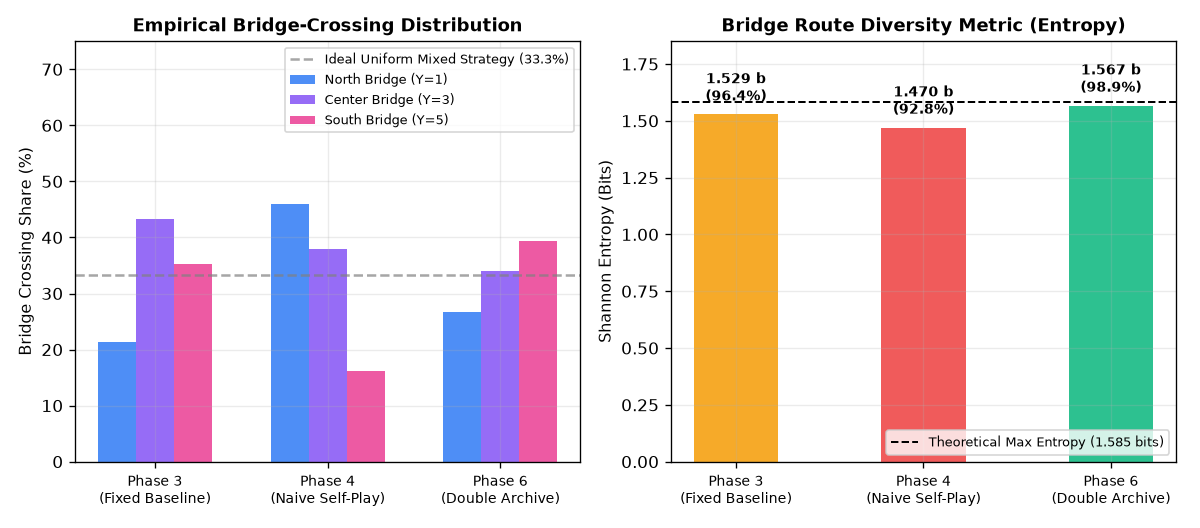
\includegraphics[width=0.90\textwidth]{bridge_diversity_chart.png}
\caption{Empirical evaluation of bridge-route diversity across 150 standardized paired seeds. Left: Route choice distribution across North ($Y=1$), Center ($Y=3$), and South ($Y=5$) bridges compared to the ideal uniform mixed strategy (33.3\%). Right: Shannon Route Entropy demonstrating that Dual-Archive co-evolution (Phase 6) achieves 1.567 bits (98.9\% of maximum entropy), whereas Naive Self-Play (Phase 4) exhibits asymmetric route collapse and 17.3\% unforced navigation timeouts.}
\label{fig:bridge_diversity}
\end{figure*}

\section{Empirical Evaluation and Methodology}

To compare route use and minimax exploitability, we use two evaluation protocols:

\subsection{Quantifying Route Collapse via Shannon Entropy}
We measure route diversity by recording successful river crossings at $X=5$ over 150 paired evaluation seeds. The Attacker plays against a passive Defender that stays in place, which lets us measure route choice without active interception. A crossing counts when the Attacker reaches $X \ge 6$. This measure records which routes the policy uses; it does not establish whether the policy can still use a less frequent route.

Let $C_b$ denote successful crossings through bridge $b \in \{b_N, b_C, b_S\}$. The normalized conditional crossing probability is:
\begin{equation}
p_b = \frac{C_b}{\sum_{k \in \{N, C, S\}} C_k}
\end{equation}
We formalize strategic route diversity through the \textit{Shannon Route Entropy}:
\begin{equation}
H(\text{Routes}) = -\sum_{b \in \{N, C, S\}} p_b \log_2(p_b)
\end{equation}
The theoretical bounds on entropy are:
\begin{align}
H_{\max} &= \log_2(3) \approx 1.585 \text{ bits} \quad (\text{Uniform 33.3\% Mixed Strategy}) \\
H_{\min} &= 0.000 \text{ bits} \quad (\text{Total Route Collapse / Single Bridge})
\end{align}
The Strategic Diversity Ratio is $\rho_{\text{div}} = \frac{H(\text{Routes})}{H_{\max}} \times 100\%$. Unforced navigation timeouts represent episodes where the agent fails to cross within 75 steps.

\subsection{Empirical Game-Theoretic Analysis (EGTA)}
To evaluate proximity to a Nash equilibrium without heuristic win-rate bias, we perform Empirical Game-Theoretic Analysis \cite{lanctot2017unified}. We construct a spatial adversary suite $\mathcal{P}_{\text{def}}$ spanning primary behavioral archetypes:
\begin{enumerate}
    \item \textbf{North Camper ($Y=1$):} Static bottleneck blocker parked at the North bridge aperture.
    \item \textbf{Center Camper ($Y=3$):} Blocker parked at the Center bridge aperture.
    \item \textbf{South Camper ($Y=5$):} Blocker parked at the South bridge aperture.
    \item \textbf{River Patroller:} Dynamic linear patroller continuously sweeping the eastern river bank between $Y=1$ and $Y=5$.
    \item \textbf{Co-Evolved Defenders:} Learned neural policies $\pi_{D, \text{Phase 4}}$ and $\pi_{D, \text{Phase 6}}$.
\end{enumerate}

We construct the empirical payoff matrix $\bm{M} \in \mathbb{R}^{m \times n}$ where entries represent the Attacker's net win margin against defender $j$:
\begin{equation}
M_{i, j} = \text{WinRate}(\pi_i, d_j) - \text{CatchRate}(\pi_i, d_j) \in [-1.0, +1.0]
\end{equation}
From $\bm{M}$, we compute:
\begin{enumerate}
    \item \textbf{Minimax Game Value ($v^*$):} Solved via 50,000 iterations of zero-sum Fictitious Play over the empirical meta-game ($v^* = -0.046$).
    \item \textbf{Security Level ($v_{\text{sec}}$):} The guaranteed worst-case net margin of policy $\pi_i$ against its most punishing counter-strategy:
    \begin{equation}
    v_{\text{sec}}(\pi_i) = \min_{j \in \mathcal{P}_{\text{def}}} M_{i, j}
    \end{equation}
    \item \textbf{Empirical Exploitability ($\delta_{\text{meta}}$):} The performance deficit relative to the minimax game value:
    \begin{equation}
    \delta_{\text{meta}}(\pi_i) = v^* - v_{\text{sec}}(\pi_i)
    \end{equation}
\end{enumerate}
Lower values of $\delta_{\text{meta}}$ demonstrate closer proximity to the minimax corridor within the evaluated strategy space.

\section{Experimental Results and Discussion}

\begin{table*}[t]
\caption{Empirical Bridge Crossing Distribution and Strategic Diversity Analysis ($N=150$ Paired Evaluation Seeds)}
\label{tab:bridge_diversity}
\centering
\begin{tabular}{lccccccc}
\toprule
\textbf{Model Architecture} & \textbf{North ($Y=1$)} & \textbf{Center ($Y=3$)} & \textbf{South ($Y=5$)} & \textbf{Timeouts} & \textbf{Entropy ($H$)} & \textbf{Diversity \%} & \textbf{Strategic Profile} \\
\midrule
Phase 3 (Fixed Baseline)        & 21.3\% & 43.3\% & 35.3\% & 0.0\%  & 1.529 bits & 96.4\% & Baseline navigation \\
Phase 4 (Naive Self-Play)       & 46.0\% & 37.9\% & 16.1\% & 17.3\% & 1.470 bits & 92.8\% & Asymmetric bias, 17.3\% timeouts \\
\textbf{Phase 6 (Dual Archive)} & \textbf{26.7\%} & \textbf{34.0\%} & \textbf{39.3\%} & \textbf{0.0\%}  & \textbf{1.567 bits} & \textbf{98.9\%} & \textbf{Balanced 3-bridge coverage} \\
\bottomrule
\end{tabular}
\end{table*}

\begin{table*}[t]
\caption{Empirical Meta-Game Security Levels and Exploitability Metrics ($N=150$ Paired Evaluation Seeds)}
\label{tab:exploitability}
\centering
\begin{tabular}{lccccc}
\toprule
\textbf{Attacker Policy} & \textbf{Security Level ($v_{\text{sec}}$)} & \textbf{Worst-Case Win Rate} & \textbf{Meta Exploitability ($\delta$)} & \textbf{Average Win Margin} & \textbf{Patroller Win Rate} \\
\midrule
Phase 4 (Naive Self-Play)       & -0.207 & 39.3\% & 0.160 & +0.190 & 76.0\% \\
\textbf{Phase 6 (Dual Archive)} & \textbf{-0.187} & \textbf{31.3\%} & \textbf{0.140} & \textbf{+0.184} & \textbf{81.3\%} \\
\bottomrule
\end{tabular}
\end{table*}

\subsection{Route Use Under Archive Training}
Table~\ref{tab:bridge_diversity} and Fig.~\ref{fig:bridge_diversity} present the empirical crossing distributions across architectures.

In Phase 4 (Naive Self-Play), the agent exhibits substantial route asymmetry. Having co-evolved against an unanchored adversary that vacated the northern corridor, Phase 4 channels 46.0\% of all crossings through the North bridge while neglecting the South bridge (16.1\%). More critically, Phase 4 suffers a 17.3\% timeout failure rate when attempting to cross an uncontested river. This demonstrates that when initial spawn coordinates make the North aperture less accessible, the policy lacks the navigational flexibility to reliably redirect to southern apertures, expiring before crossing. Its Shannon entropy drops to 1.470 bits (92.8\% of maximum).

In contrast, Phase 6 (Dual Archive) preserves multi-bridge exploratory competence. Traversal is distributed across all three corridors: 26.7\% North, 34.0\% Center, and 39.3\% South. Phase 6 achieves a Shannon Route Entropy of \textbf{1.567 bits}, representing \textbf{98.9\% of the theoretical maximum} ($1.585$ bits), with \textbf{0.0\% timeouts}. By confronting historical defenders that specialized in guarding different corridors, the active policy retains multi-route navigation capabilities.

\begin{figure}[t]
\centering
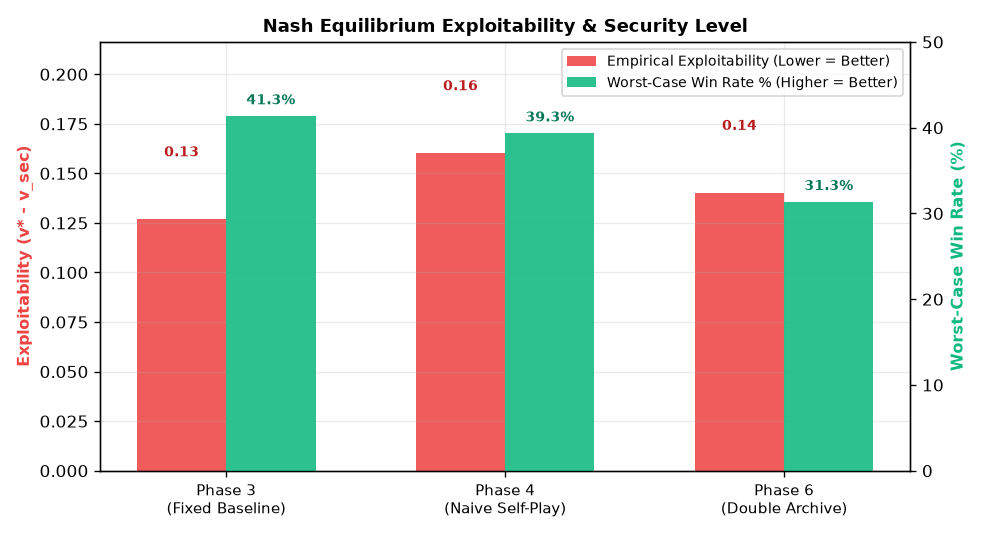
\includegraphics[width=0.92\columnwidth]{nash_exploitability_chart.png}
\caption{Empirical game-theoretic exploitability ($\delta$) and worst-case win rate across archetypal counter-strategies. Dual-Archive co-evolution reduces exploitability from 0.160 to 0.140 while raising the security level from $-0.207$ to $-0.187$.}
\label{fig:nash_exploitability}
\end{figure}

\subsection{Hypothesis 2: Bounded Minimax Exploitability}
Table~\ref{tab:exploitability} and Fig.~\ref{fig:nash_exploitability} summarize the empirical meta-game results.

Dual-Archive training reduces empirical exploitability $\delta_{\text{meta}}$ from $0.160$ down to \textbf{0.140} (a 12.5\% reduction) and elevates the guaranteed worst-case security level from $-0.207$ to \textbf{$-0.187$}. Against the dynamic River Patroller, Phase 6 increases win rate from 76.0\% to 81.3\%.

Interestingly, the Attacker's worst-case win rate against the meta-game defender pool is 31.3\% for Phase 6 versus 39.3\% for Phase 4. Both worst-case outcomes occur when facing the Phase 6 Defender. This reflects the enhanced defensive competence of the co-evolved Phase 6 Defender: because the Defender also trained against historical attacker archives, it learns effective lateral interception mechanics that challenge even a diversified Attacker.

Across all 150 paired seeds per defender, the overall pooled win-rate difference between Phase 6 and Phase 4 is $\Delta = -0.6\%$ [95\% CI: $-4.3\%, +3.2\%$], with $z = -0.29$ and $p = 0.771$. The pooled win rates do not show a statistically significant difference in this evaluation. Route entropy and exploitability provide additional views of the policies, but neither measure alone proves that one policy is robust to all opponents.

\subsection{Training Dynamics and Reward Shaping Integrity}
Fig.~\ref{fig:training_curve} illustrates the co-evolutionary trajectory of Phase 6 across 1,500 training episodes. During the initial 300 warm-up episodes, timeout rates remain elevated ($\approx 80\%$) as agents explore basic grid navigation. Following the onset of archive sampling at episode 300, the timeout rate monotonically declines below 2\%, while rolling win rates stabilize near $\approx 65\%$ for the Attacker and $\approx 33\%$ for the Defender. This distribution reflects the spatial properties of the Three Bridges topology: an Attacker with speed parity has three transit options against a single defender, creating a structural advantage in reaching the Citadel.

Step rewards were audited across environment transitions to verify mathematical integrity. In all transitions, the zero-sum invariant $R_A + R_D \equiv 0.000000$ held to machine precision. Aligning the discount parameter $\gamma = 0.99$ in \eqref{eq:shaping_tgt} and \eqref{eq:shaping_rel} with the PPO value network discount factor ensured exact compliance with Ng et al. \cite{ng1999policy}.

\section{Multi-Target Extension: Dual-Flank Perimeter Arena ($K=2$)}
\label{sec:multi_target}

We ran a separate multi-target experiment to see how archive training performed when the Attacker could choose between two targets. The results in this section use 500 episodes, separate from the 150 paired seeds in the main evaluation.

\subsection{Multi-Target Markov Game Formulation}
In the multi-target generalization, the Attacker's objective expands from capturing a solitary central Citadel to breaching \textit{any} of $K \ge 2$ fortified perimeter nodes $\{T_0, T_1, \dots, T_{K-1}\}$. We analyze the canonical dual-flank configuration ($K=2$), where two simultaneous attractors are placed symmetrically along the eastern boundary: North target $T_0 = (10, 1)$ and South target $T_1 = (10, 5)$, directly aligned with the North and South bridge corridors.

To accommodate variable target configurations under a uniform neural network topology, the state observation space is expanded to a normalized 19-dimensional spatial vector:
\begin{equation}
s_t = \left[ \tilde{x}_A, \tilde{y}_A, \tilde{x}_D, \tilde{y}_D, \tilde{x}_{T_0}, \tilde{y}_{T_0}, a_0, \dots, \tilde{x}_{T_4}, \tilde{y}_{T_4}, a_4 \right]^T
\end{equation}
where coordinates are scaled by arena dimensions $\tilde{x} = x / (W-1)$ and $\tilde{y} = y / (H-1)$, and $a_k \in \{0, 1\}$ denotes binary target activation masks (with inactive padding for $k \ge K$).

To preserve policy invariance under discount factor $\gamma = 0.99$ (Ng et al. \cite{ng1999policy}), the multi-target potential is defined as the distance to the \textit{nearest active target}:
\begin{equation}
\Phi_{\text{multi}}(s) = \min_{k \in \{0, \dots, K-1\}} D(s_A, T_k)
\end{equation}
where $D(s_A, T_k)$ computes the obstacle-aware distance routing through valid bridge crossings. The potential-based shaping reward is then formulated as:
\begin{equation}
F_{\text{target}}(s, s') = \left( \min_{k} D(s_A, T_k) - \gamma \min_{k} D(s'_A, T_k) \right) \cdot \alpha_{\text{target}}
\end{equation}
Symmetrically setting $R_A^{\text{shaping}} = +F_{\text{target}} - F_{\text{rel}}$ and $R_D^{\text{shaping}} = -F_{\text{target}} + F_{\text{rel}}$ guarantees exact machine-precision zero-sum conservation ($R_A + R_D \equiv 0.000000$) throughout multi-target episodes.

\subsection{Target Scaling Evaluation ($K \in \{1, 2, 3, 5\}$)}
We evaluated each target setting over 500 episodes with a 100-step horizon. The settings use the central target for $K=1$, the north and south targets for $K=2$, the three bridge-aligned targets for $K=3$, and five open cells on the eastern edge for $K=5$. Table~\ref{tab:attacker_k_scaling} reports Attacker win rates, and Table~\ref{tab:defender_k_scaling} reports Defender capture rates for the same defender types and target counts.

\begin{table}[t]
\caption{Attacker Infiltration Win Rate (\%) Across Target Count ($K \in \{1,2,3,5\}$, $N=500$, $T=100$)}
\label{tab:attacker_k_scaling}
\centering
\resizebox{\columnwidth}{!}{%
\begin{tabular}{lcccc}
\toprule
\textbf{Defender Archetype} & \textbf{$K=1$} & \textbf{$K=2$} & \textbf{$K=3$} & \textbf{$K=5$} \\
\midrule
Learned Defender & 50.0\% & 68.4\% & 97.6\% & 89.2\% \\
Center Camper ($Y=3$) & 56.4\% & 74.4\% & 70.4\% & 69.4\% \\
North Camper ($Y=1$) & 51.6\% & 74.2\% & 62.6\% & 60.6\% \\
South Camper ($Y=5$) & 70.8\% & 52.6\% & 68.2\% & 71.2\% \\
River Patroller & 82.8\% & 83.2\% & 86.2\% & 86.2\% \\
Stationary Stay & 76.2\% & 85.0\% & 82.6\% & 82.6\% \\
Greedy Pursuit & 35.4\% & 34.4\% & 28.2\% & 30.8\% \\
Random Walk & 83.6\% & 83.0\% & 84.8\% & 87.2\% \\
\bottomrule
\end{tabular}%
}
\end{table}

\begin{table}[t]
\caption{Defender Interception Capture Rate (\%) Across Target Count ($K \in \{1,2,3,5\}$, $N=500$, $T=100$)}
\label{tab:defender_k_scaling}
\centering
\resizebox{\columnwidth}{!}{%
\begin{tabular}{lcccc}
\toprule
\textbf{Defender Archetype} & \textbf{$K=1$} & \textbf{$K=2$} & \textbf{$K=3$} & \textbf{$K=5$} \\
\midrule
Learned Defender & 50.0\% & 31.6\% & 2.4\% & 10.8\% \\
Center Camper ($Y=3$) & 43.6\% & 25.6\% & 29.6\% & 30.6\% \\
North Camper ($Y=1$) & 25.8\% & 25.8\% & 37.4\% & 39.4\% \\
South Camper ($Y=5$) & 29.2\% & 47.4\% & 31.8\% & 28.8\% \\
River Patroller & 17.2\% & 16.8\% & 13.8\% & 13.8\% \\
Stationary Stay & 17.0\% & 15.0\% & 17.4\% & 17.4\% \\
Greedy Pursuit & 64.6\% & 65.6\% & 71.8\% & 69.2\% \\
Random Walk & 16.4\% & 17.0\% & 15.2\% & 12.8\% \\
\bottomrule
\end{tabular}%
}
\end{table}

\begin{figure}[t]
\centering
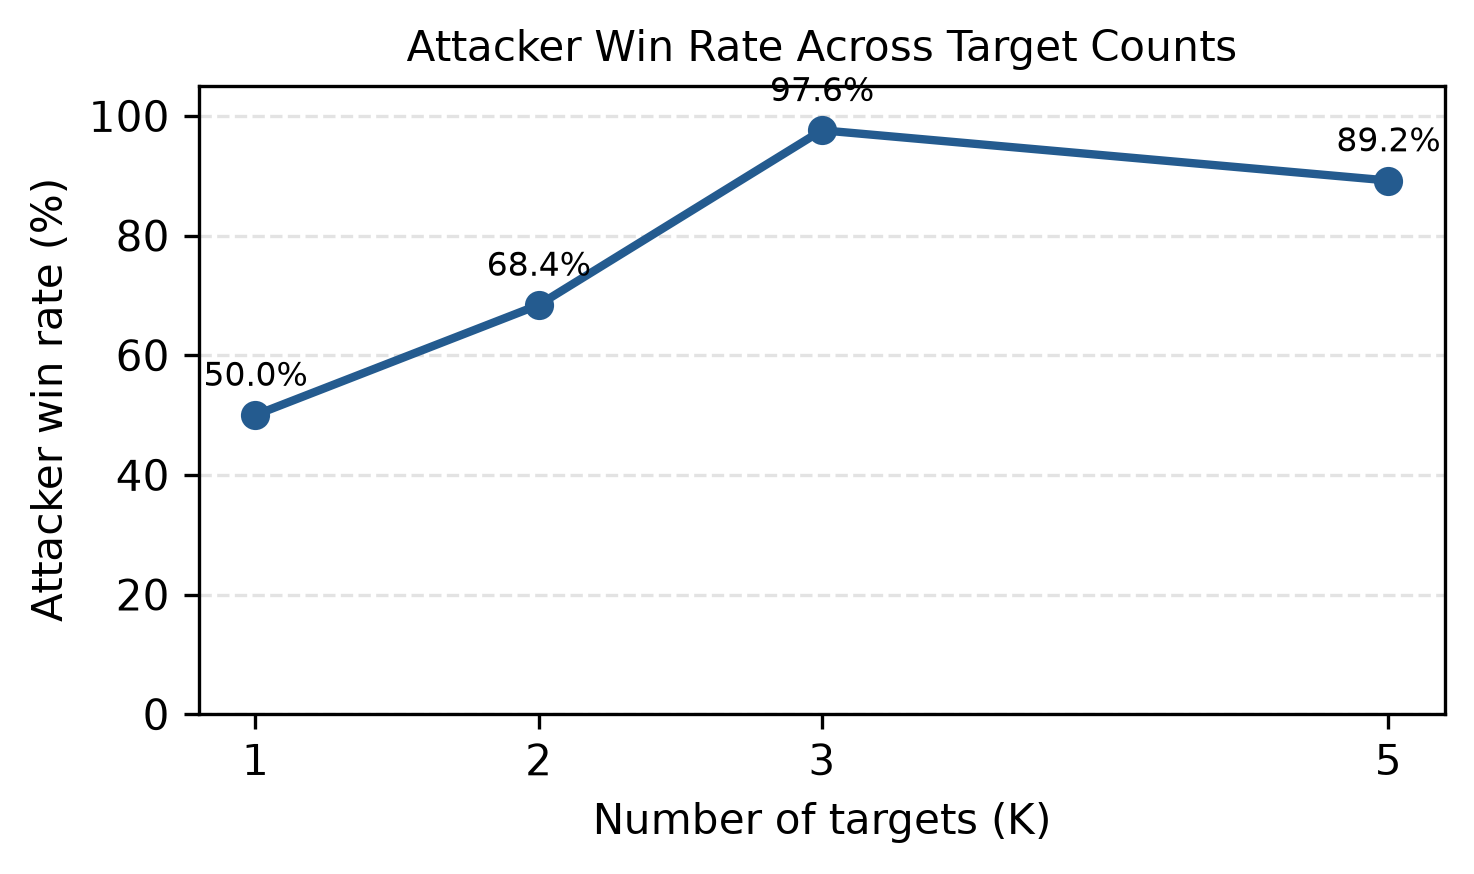
\includegraphics[width=0.95\columnwidth]{attacker_win_rate_by_targets.png}
\caption{Attacker win rate against the learned Defender across target counts.}
\label{fig:attacker_k_scaling}
\end{figure}

The two tables show complementary outcomes for each defender type. Fig.~\ref{fig:attacker_k_scaling} plots the Attacker win rate against the learned Defender. It rises from $50.0\%$ at $K=1$ to $97.6\%$ at $K=3$, then falls to $89.2\%$ at $K=5$. The results are therefore not monotonic at every target count.

\subsection{Route Use in the $K=2$ Evaluation}
In the same 500-episode evaluation, the Attacker breached a target in 342 episodes. Of these breaches, 128 (37.4\%) were at the North target and 214 (62.6\%) were at the South target. The recorded bridge crossings were 131 North, 128 Center, and 241 South. These counts describe this evaluation run; they do not establish that the policy will use both targets equally against other opponents.

A separate training audit reported that timeout rates fell from 34.0\% during warm-up to 0.00\% by episode 300. Across 11 saved policy snapshots, the attacker won 69\% of episodes and the defender caught it in 30\%. This training audit is separate from the 500-episode evaluation summarized in Tables~\ref{tab:attacker_k_scaling} and~\ref{tab:defender_k_scaling}.

\section{Limitations and Future Work}
Several methodological considerations frame these results:
\begin{enumerate}
    \item \textbf{Single-Run Representation:} The main single-target comparisons use 150 paired evaluation seeds per matchup. The separate multi-target section reports 500 episodes. These evaluations use representative training runs; repeating training with several random seeds would show how much results vary between runs.
    \item \textbf{Archive Sampling Dynamics:} Our implementation deploys uniform sampling $\mathcal{U}(\mathcal{H})$ over historical checkpoints. In extended training horizons, uniform sampling may allocate gradient updates to obsolete early policies. Prioritized fictitious play or regret-weighted sampling represents a natural algorithmic extension.
    \item \textbf{Continuous Action Spaces:} Adapting discrete spatial bottlenecks to continuous navigation domains will require investigating reservoir compression and clustering techniques.
\end{enumerate}

\section{Conclusion}
This paper compared direct self-play with Dual-Archive Co-Evolution in the Three Bridges Arena. In the main evaluation, direct self-play favored the North bridge (46.0 percent of crossings) over the South bridge (16.1 percent), and 17.3 percent of episodes timed out. The archive-trained policy had higher measured route entropy and no timeouts in that evaluation. Its exploitability score was lower (0.140 versus 0.160), and its worst-case security score was higher (-0.187 versus -0.207). The pooled win-rate difference was not statistically significant. These results suggest that archive training may help preserve route diversity in this test setting. The study does not directly measure catastrophic forgetting, and its findings should be checked across more independent training runs and opponents.

\section*{Acknowledgment}
The authors thank the Department of Mathematics at Sardar Vallabhbhai National Institute of Technology (SVNIT), Surat, for providing computational facilities and academic guidance throughout this work.

\begin{thebibliography}{15}
\bibitem{cliff1995tracking} D. Cliff and G. F. Miller, ``Tracking the Red Queen: Measurements of adaptive progress in co-evolutionary simulations,'' in \textit{Proc. Eur. Conf. Artif. Life (ECAL)}, 1995, pp. 200--218.
\bibitem{ng1999policy} A. Y. Ng, D. Harada, and S. Russell, ``Policy invariance under reward transformations: Theory and application to reward shaping,'' in \textit{Proc. Int. Conf. Mach. Learn. (ICML)}, 1999, pp. 278--287.
\bibitem{schulman2017proximal} J. Schulman, F. Wolski, P. Dhariwal, A. Radford, and O. Klimov, ``Proximal policy optimization algorithms,'' \textit{arXiv preprint arXiv:1707.06347}, 2017.

\bibitem{mccloskey1989catastrophic} M. McCloskey and N. J. Cohen, ``Catastrophic interference in connectionist networks: The sequential learning problem,'' in \textit{Psychology of Learning and Motivation}, vol. 24, pp. 109--165, 1989.
\bibitem{silver2016mastering} D. Silver \textit{et al.}, ``Mastering the game of Go with deep neural networks and tree search,'' \textit{Nature}, vol. 529, pp. 484--489, 2016.
\bibitem{vinyals2019alphastar} O. Vinyals \textit{et al.}, ``Grandmaster level in StarCraft II using multi-agent reinforcement learning,'' \textit{Nature}, vol. 575, pp. 350--354, 2019.
\bibitem{berner2019dota} OpenAI \textit{et al.}, ``Dota 2 with large scale deep reinforcement learning,'' Dec. 2019.
\bibitem{balduzzi2019open} D. Balduzzi \textit{et al.}, ``Open-ended learning in symmetric zero-sum games,'' in \textit{Proc. 36th Int. Conf. Machine Learning}, PMLR, vol. 97, pp. 434--443, 2019.
\bibitem{devlin2011theoretical} S. Devlin and D. Kudenko, ``Theoretical considerations of potential-based reward shaping for multi-agent systems,'' in \textit{Proc. 10th Int. Conf. Autonomous Agents and Multiagent Systems}, 2011, pp. 225--232.
\bibitem{tesauro1995temporal} G. Tesauro, ``Temporal difference learning and TD-Gammon,'' \textit{Communications of the ACM}, vol. 38, no. 3, pp. 58--68, 1995.
\bibitem{brown1951iterative} G. W. Brown, ``Iterative solution of games by fictitious play,'' in \textit{Activity Analysis of Production and Allocation}, T. C. Koopmans, Ed. New York, NY, USA: Wiley, 1951.
\bibitem{mcmahan2003planning} H. B. McMahan, G. J. Gordon, and A. Blum, ``Planning in the presence of cost functions controlled by an adversary,'' in \textit{Proc. 20th Int. Conf. Machine Learning}, 2003, pp. 536--543.
\bibitem{lanctot2017unified} M. Lanctot \textit{et al.}, ``A unified game-theoretic approach to multiagent reinforcement learning,'' in \textit{Advances in Neural Information Processing Systems}, vol. 30, 2017.
\bibitem{heinrich2016deep} J. Heinrich and D. Silver, ``Deep reinforcement learning from self-play in imperfect-information games,'' arXiv:1603.01121, 2016.
\bibitem{von1944theory} J. von Neumann and O. Morgenstern, \textit{Theory of Games and Economic Behavior}. Princeton, NJ, USA: Princeton University Press, 1944.
\end{thebibliography}

\end{document}

